\documentclass{standalone}
%
\usepackage{tikz}
\usetikzlibrary{backgrounds,arrows.meta,shapes.callouts}
\usepackage{xcolor}
%
\definecolor{space}{HTML}{1F2C4E}
\definecolor{earth}{HTML}{0089FA}
\definecolor{dida}{HTML}{FFDE00}
\definecolor{title}{HTML}{FBA706}
\definecolor{galaxy}{HTML}{4278A4}
\definecolor{paper01}{HTML}{BE8A3F}
\definecolor{paper02}{HTML}{E5D09B}
%
\usepackage{fontspec}
\setmainfont{Open Dyslexic}
%
\title{Vite tra le stelle}
\begin{document}
	\begin{tikzpicture}[background rectangle/.style={fill=white},show background rectangle,>={[inset=0,angle'=27]Stealth}]
		% title
		\draw [black,ultra thick,fill=title] (0,12.8) rectangle (30,16.8);
		\node at (15,14.8) {\textcolor{black}{\fontsize{75}{76}\selectfont Vite tra le stelle}};
		% stripe
		\begin{scope}[shift={(0,12)}]
			\draw [fill=earth!50!white, thick] (14.5,0) rectangle (26.5,-127.5);
			\foreach \i in {0,1,...,11}
			{
				\draw [fill=white, thick] (14.75+\i,-0.5) rectangle (15.25+\i,-1);
			}
			%
			\foreach \j in {0,1,...,11}
			{
				\draw [fill=white, thick] (14.75+\j,-126.5) rectangle (15.25+\j,-127);
			}
		\end{scope}
		%
		% Marguerite de la Sablière
		%
		\begin{scope}[shift={(0,8)}]
			\draw [fill=earth!50!space, thick] (3,0.8) rectangle (13,-10.8);
			\node at (8,-5) {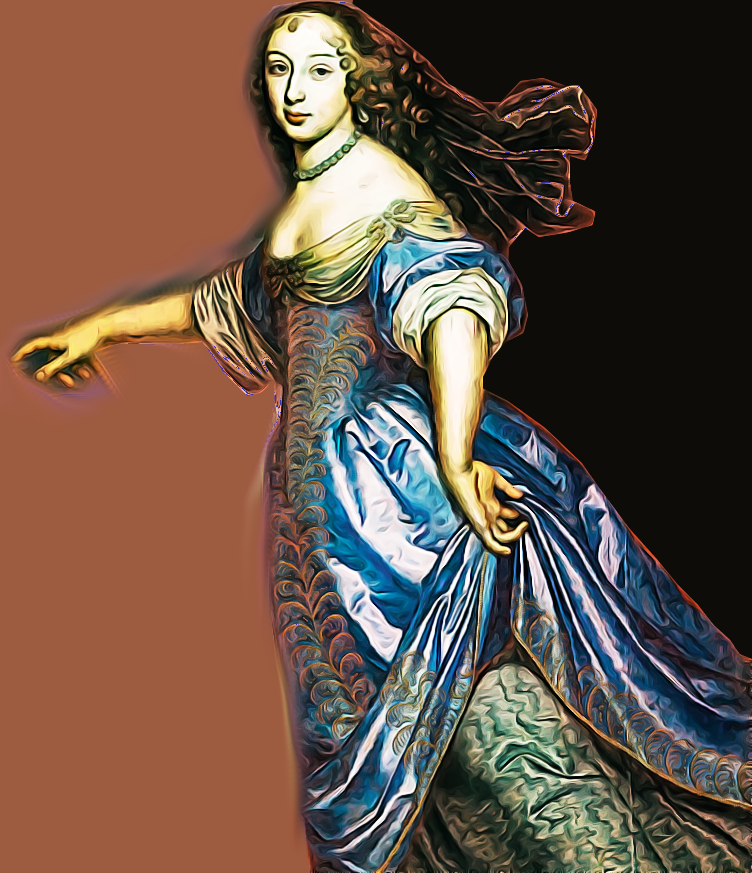
\includegraphics[width=10cm]{img/2024/marguerite}};
			%
			\draw [fill=galaxy, ultra thick] (3.5,-10.3) rectangle (12.5,-11.4);
			\node at (8,-10.9) {\textcolor{black}{\fontsize{18}{19}\selectfont Marguerite de la Sablière}};
			%
			\draw [fill=title, thick] (14,0.9) rectangle (27,1.8);
			\node (example-textwidth-2) [right, align=left, text width=12cm, color=black, font=\fontsize{18pt}{19pt}\selectfont] at (15,1.3) {\textbf{1640}};
			%
			\node (example-textwidth-2) [right, align=left, text width=12cm, color=black, font=\fontsize{18pt}{19pt}\selectfont] at (15,-0.1) {Donna universale};
			%
			\draw [fill=dida, thick] (14,-1) rectangle (27,-20);
			\node (example-textwidth-2) [right, align=left, text width=11cm, color=black, font=\fontsize{18pt}{19pt}\selectfont] at (15,-10.5) {Ricevette un'educazione vasta e abbastanza inconsueta per una donna dell'epoca. Studiò, infatti, latino, matematica, fisica e anatomia. Tra i suoi insegnanti si contano \textbf{Joseph Sauveur} e \textbf{Gilles Personne de Roberval } con i quali studiò matematica, fisica e anche astronomia.\\In un'epoca in cui andavano di gran moda i salotti letterari, Mme de la Sablière aprì la sua casa alla discussione scientifica, in pratica un salotto scientifico.\\Provò anche a cimentarsi nell'astronomia osservando il pianeta Giove. I suoi sforzi vennero derisi dal critico \textbf{Nicolas Boileau-Despréaux} nel \emph{pamphlet} \emph{Satire contre les femmes}. In sua difessa scrisse però \textbf{Charles Perrault} in \emph{Apologie des femmes}, a testimonianza del rispetto che aveva ottenuto.\\Spese anche parte della sua vita nell'ospitare gli incurabili.};
			%
			\draw [fill=title, thick] (14,-20.8) rectangle (27,-21.8);
			\node (example-textwidth-2) [right, align=left, text width=12cm, color=black, font=\fontsize{18pt}{19pt}\selectfont] at (15,-21.3) {\textbf{8 gennaio 1693}};
		\end{scope}
		%
		% Claudine Picardet
		%
		\begin{scope}[shift={(0,-24.5)}]
			\foreach \i in {0,1,...,11}
			{
				\draw [fill=white, thick] (14.75+\i,9) rectangle (15.25+\i,9.5);
			}
			%
			\draw [fill=earth!50!white, thick] (3,6.75) rectangle (13,-11.55);
			\node at (8,-2.4) {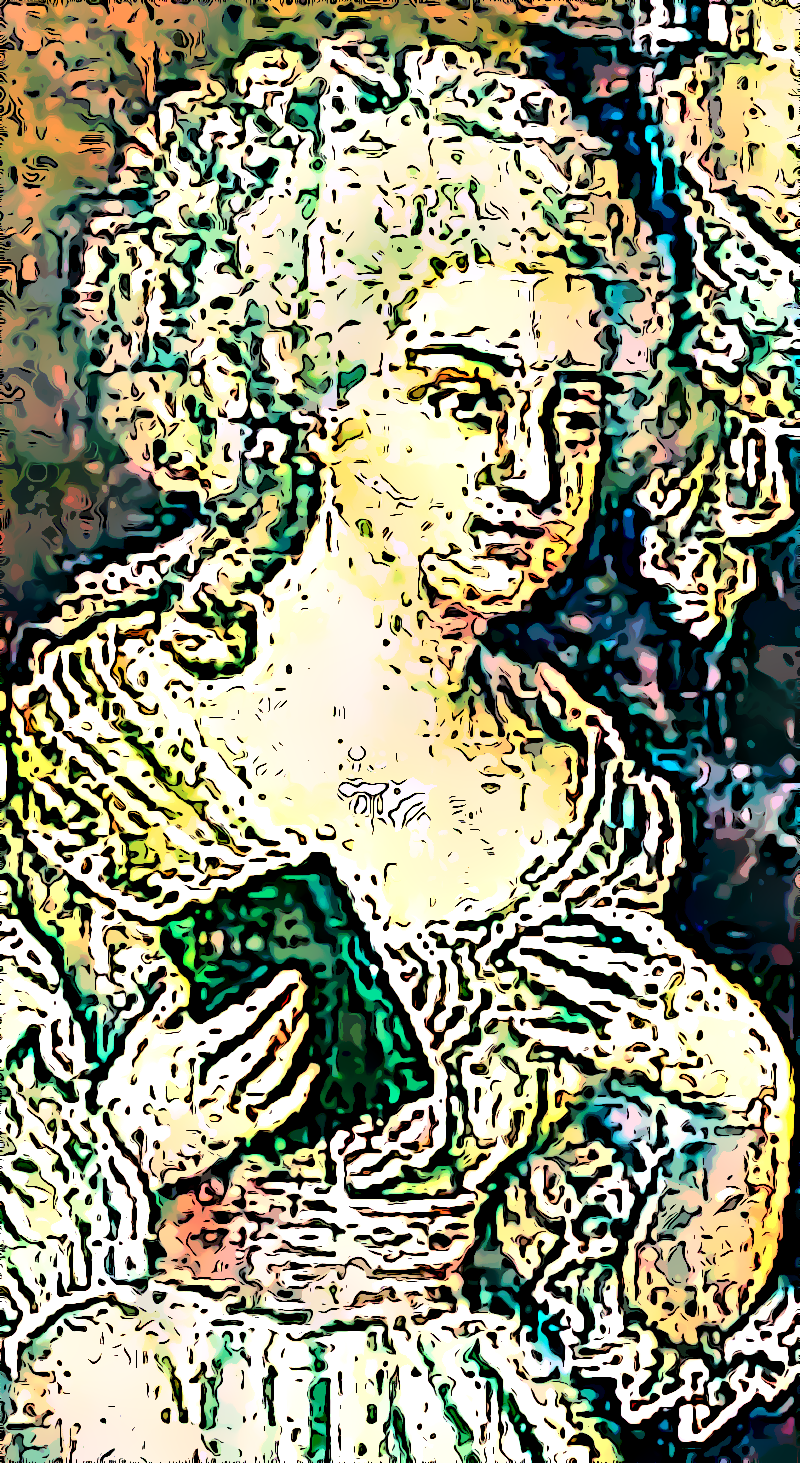
\includegraphics[width=10cm]{img/2024/picardet}};
			%
			\draw [fill=galaxy, ultra thick] (4.6,-11) rectangle (11.4,-12);
			\node at (8,-11.5) {\textcolor{black}{\fontsize{18}{19}\selectfont Claudine Picardet}};
			%
			\draw [fill=title, thick] (14,6.85) rectangle (27,7.75);
			\node (example-textwidth-2) [right, align=left, text width=12cm, color=black, font=\fontsize{18pt}{19pt}\selectfont] at (15,7.35) {\textbf{7 agosto 1735}};
			%
			\node (example-textwidth-2) [right, align=left, text width=11cm, color=black, font=\fontsize{18pt}{19pt}\selectfont] at (15,5.5) {Chimica, mineralologa, meteorologa e traduttrice scientifica};
			%
			\draw [fill=dida, thick] (14,4.2) rectangle (27,-12.6);
			\node (example-textwidth-2) [right, align=left, text width=10cm, color=black, font=\fontsize{18pt}{19pt}\selectfont] at (15,-4.3) {E' nota soprattutto per le molte traduzioni di lavori scientifici dallo svedese, inglese, tedesco e italiano al francese. In particolare era particolarmente nota e apprezzata la sua traduzione dei lavori del chimico \textbf{Carl Wilhelm Scheele}.\\Sebbene si sia interessata soprattutto alla chimica e alla mineralogia, ha anche tradotto alcune opere nel campo della meteorologia con attinenze astronomiche come \emph{Observationes astron. annis 1781, 82, 83 institutæ in observatorio regio Havniensi} del 1784 in cui sono riportate le osservazioni astronomiche di \textbf{Thomas Bugge} su alcune longitudini marziane. La sua traduzione venne pubblicata nel 1787 sul \emph{Journal des savants}.};
			%
			\node (example-textwidth-2) [right, align=left, text width=11cm, color=black, font=\fontsize{18pt}{19pt}\selectfont] at (15,-18.5) {Per migliorare le sue competenze nella traduzione dei lavori scientifici, applicò, in pratica, il metodo scientifico, riproducendo gli esperimenti di cui traduceva i risultati. Questo metodo di lavoro emerge in particolare nella traduzione dei neologismi utilizzati da \textbf{Abraham Gottlob Werner}.\\Nal 1785 ha eseguito una serie di misure barometriche che vennero successivamente presentate da \textbf{Antoine Lavoisier} presso l'Accademnia delle Scienze di Parigi.};
			%
			\draw [fill=title, thick] (14,-24.6) rectangle (27,-25.6);
			\node (example-textwidth-2) [right, align=left, text width=12cm, color=black, font=\fontsize{18pt}{19pt}\selectfont] at (15,-25) {\textbf{4 ottobre 1820}};
		\end{scope}
		%
		% Wang Zhenyi
		%
		\begin{scope}[shift={(0,-60.7)}]
			\foreach \i in {0,1,...,11}
			{
				\draw [fill=white, thick] (14.75+\i,8.8) rectangle (15.25+\i,9.3);
			}
			%
			\draw [thick] (3,6.5) rectangle (13,-7.3);
			\node at (8,-0.4) {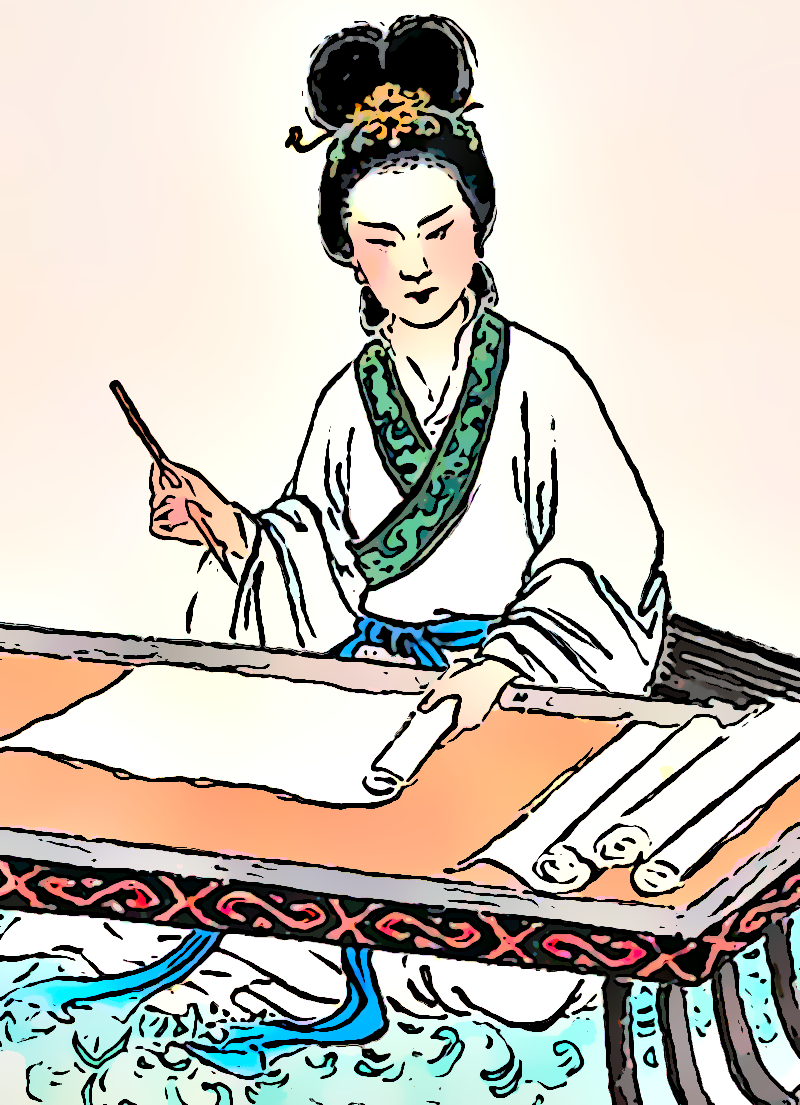
\includegraphics[width=10cm]{img/2024/wang_zhenyi}};
			%
			\draw [fill=galaxy, ultra thick] (5.3,-6.8) rectangle (10.7,-7.8);
			\node at (8,-7.3) {\textcolor{black}{\fontsize{18}{19}\selectfont Wang Zhenyi}};
			%
			\draw [fill=title, thick] (14,6.55) rectangle (27,7.45);
			\node (example-textwidth-2) [right, align=left, text width=12cm, color=black, font=\fontsize{18pt}{19pt}\selectfont] at (15,6.95) {\textbf{1768}};
			%
			\node (example-textwidth-2) [right, align=left, text width=10cm, color=black, font=\fontsize{18pt}{19pt}\selectfont] at (15,5.6) {Astronoma, matematica, poetessa};
			%
			\draw [fill=dida, thick] (14,4.5) rectangle (27,-6.1);
			\node (example-textwidth-2) [right, align=left, text width=10cm, color=black, font=\fontsize{18pt}{19pt}\selectfont] at (15,-0.8) {Come una stella di grande massa che vive la sua vita bruciando le tappe, anche Wang Zhenyi ha vissuto brevemente, appena 29 anni, riuscendo però a illuminare l'astronomia e la matematica cinese. Uno dei suoi più bei risultati è stata la spiegazione e la dimostrazione della precessione degli equinozi, nonché la proposizione di un metodo per prevedere tale fenomeno.};
			%
			\node (example-textwidth-2) [right, align=left, text width=11cm, color=black, font=\fontsize{18pt}{19pt}\selectfont] at (15,-11.6) {Nei suoi saggi ha toccato argomenti come le eclissi lunari e il legame tra queste ultime e le eclissi di Sole, su cui ha anche condotto alcuni esperimenti. Ha inoltre fornito le sue considerazioni sui moti dei pianeti e si è interessata dell'astronomia del calendario, che all'epoca era ritenuta troppo complessa sia dagli astronomi orientali sia da quelli occidentali. E' soprattutto in questo campo specifico che ha affrontato delle forti restrizioni in quanto donna.};			
			%
			\shade [bottom color=paper02,top color=paper01] (14,-17) rectangle (27,-21.6);
			\draw [thick] (14,-17) rectangle (27,-21.6);
			\node (example-textwidth-2) [right, align=left, text width=11cm, color=black, font=\fontsize{18pt}{19pt}\selectfont] at (15,-19.2) {E' un dato di fatto:\\le Donne sono identiche agli Uomini.\\Non sei convinto,\\che le tue Figlie possono essere eroiche?};
			%
			\draw [fill=title, thick] (14,-22.3) rectangle (27,-23.2);
			\node (example-textwidth-2) [right, align=left, text width=12cm, color=black, font=\fontsize{18pt}{19pt}\selectfont] at (15,-22.8) {\textbf{1797}};
		\end{scope}
		%
		% Margaret Bryan
		%
		\begin{scope}[shift={(0,-91.5)}]
			\foreach \i in {0,1,...,11}
			{
				\draw [fill=white, thick] (14.75+\i,6.4) rectangle (15.25+\i,5.9);
			}
			%
			\draw [thick] (3,3.95) rectangle (13,-8.55);
			\node at (8,-2.3) {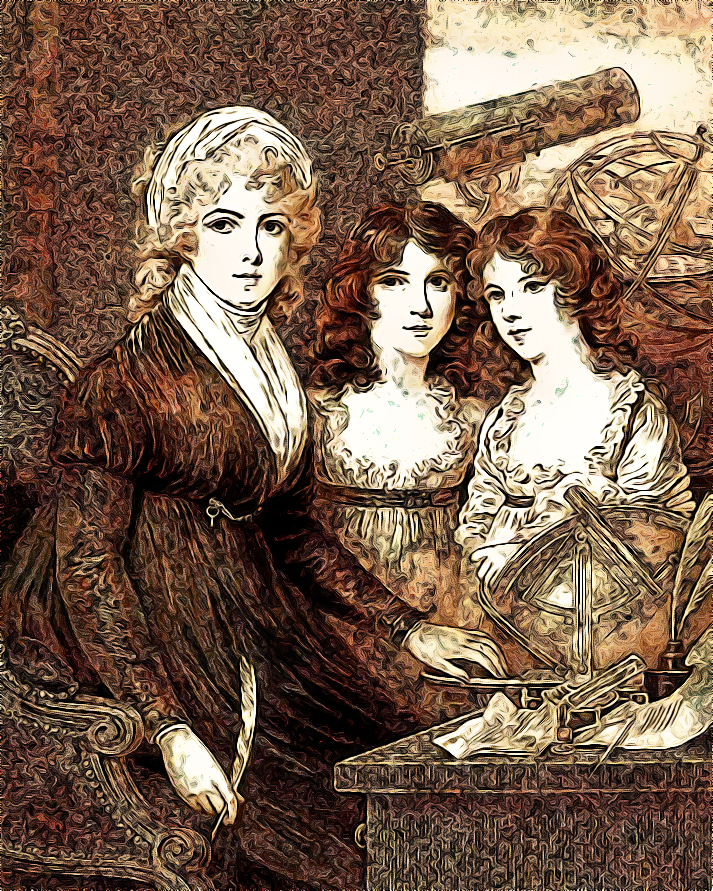
\includegraphics[width=10cm]{img/2024/margaret_bryan}};
			%
			\draw [fill=galaxy, ultra thick] (5.2,-8) rectangle (10.8,-9);
			\node at (8,-8.5) {\textcolor{black}{\fontsize{18}{19}\selectfont Margaret Bryan}};
			%
			\draw [fill=title, thick] (14,3.95) rectangle (27,4.85);
			\node (example-textwidth-2) [right, align=left, text width=12cm, color=black, font=\fontsize{18pt}{19pt}\selectfont] at (15,4.35) {\textbf{1759}};
			%
			\node (example-textwidth-2) [right, align=left, text width=10cm, color=black, font=\fontsize{18pt}{19pt}\selectfont] at (15,3) {Insegnante};
			%
			\draw [fill=dida,thick] (14,2.2) rectangle (27,-5.2);
			\node (example-textwidth-2) [right, align=left, text width=11cm, color=black, font=\fontsize{18pt}{19pt}\selectfont] at (14.8,-1.5) {Ha raccolto le sue lezioni in una serie di libri di testo. Il suo primo libro, \emph{Compendious System of Astronomy} pubblicato nel 1797, era dedicato ai suoi studenti. Nel frontespizio la troviamo ritratta insieme con le sue due figlie, circondata da alcuni strumenti astronomici, come un telescopio o un astrolabio.};
			%
			\node (example-textwidth-2) [right, align=left, text width=11cm, color=black, font=\fontsize{18pt}{19pt}\selectfont] at (15,-7.4) {Nel 1806 vennero pubblicate le sue \emph{Lectures on Natural Philosophy}, una raccolta di 13 lezioni su idrostatica, ottica, pneumatica e acustica.};
			%
			\draw [fill=dida, thick] (14,-9.7) rectangle (27,-19.9);
			\node (example-textwidth-2) [right, align=left, text width=11cm, color=black, font=\fontsize{18pt}{19pt}\selectfont] at (15,-14.8) {Nel 1815, esce \emph{Astronomical and Geographical Class Book for Schools}. Il testo era precedentemente disponibile solo per nobili, insegnanti e venditori di libri. Proprio come i moderni libri di testo, era corredato di diagrammi esplicativi e di esercizi. Si occupava di vari problemi di meccanica (la meccanica del fucile o del pallone ad aria calda, per esempio), includendo anche i lavori di \textbf{Isaac Newton}, \textbf{Galileo Galilei} e \textbf{Benjamin Franklin}.};
			%
			\draw [fill=title, thick] (14,-20.6) rectangle (27,-21.6);
			\node (example-textwidth-2) [right, align=left, text width=12cm, color=black, font=\fontsize{18pt}{19pt}\selectfont] at (15,-21.1) {\textbf{1836}};
		\end{scope}
		% image credits
		\begin{scope}[shift={(0,-117)}]
			\draw [fill=space,thick] (2,1) rectangle (28,-1);
			%
			\node (example-textwidth-2) [right, align=left, text width=25cm, color=white, font=\fontsize{18pt}{19pt}\selectfont] at (2.5,0) {Le immagini sono tratte da Wikipedia o da Women in History e poi rielaborate graficamente usando il filtro G'MIC-Qt di Gimp.};
		\end{scope}
		%
		\begin{scope}[shift={(0,-119)}]
			\node at (27,0) () {
\includegraphics[width=3.7cm]{licenza}};
			\node (example-textwidth-2) [right, align=left, text width=14cm, color=black, font=\fontsize{14pt}{15pt}\selectfont] at (12.5,-0.1) {Testo e grafica: @ulaulaman - Gianluigi Filippelli};
		\end{scope}
	\end{tikzpicture}
\end{document}
